  \subsubsection{Асимметричный случай отражения}
  На рисунке \ref{ris:assymetric_exp_50}
  приведены результаты двухкристального эксперимента, где в качестве
  кристалла образца и монохроматора использовался кристалл кремния Si(440). Образец был взят таким
  образом, что плоскость отражения располагалась под углом $\phi = 20^o 53^{'}$ к поверхности.

  \begin{figure}[H]
    \centering
    \subfloat[]{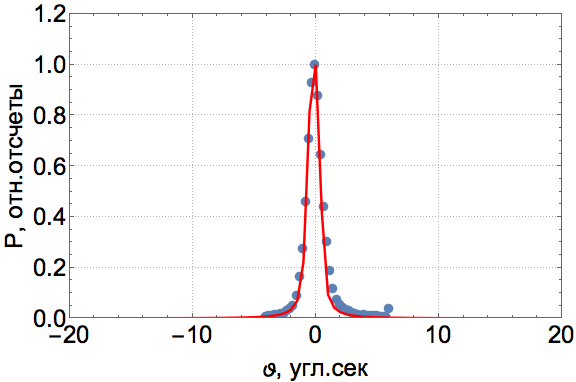
\includegraphics[width=0.45\textwidth]{images/assym-blue-50.png}\label{ris:assymetric_exp_a}}
    \hfill
    \subfloat[]{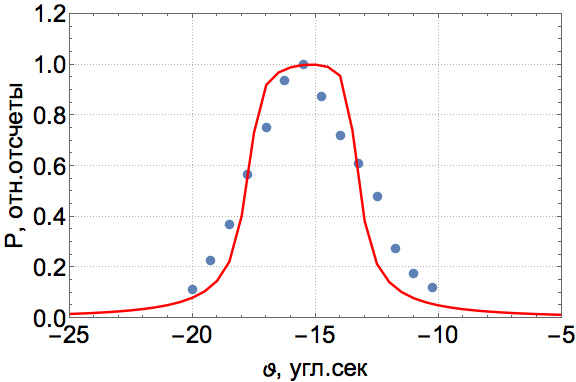
\includegraphics[width=0.45\textwidth]{images/assym-red-50.png}\label{ris:assymetric_exp_b}}
    \caption{Двухкристальная КДО для схемы с установленным кристаллом монохроматором Si(440) и асимметричным образцом Si(440),
    угол разориентации поверхности $\varphi = 20^o53^{'}$ для разных углов падения (a) $b = 33.52$, $\varphi$ > 0, (b) $b = 0.03$, $\varphi$ < 0.
     Размер щелевых устройств $S_1 = S_2 = 50$ мкм}
    \label{ris:assymetric_exp_50}
  \end{figure}

  % Как было показано в разделе \ref{sec:rocking_curve_section}, чтобы получить
  % рентгеновский пучок с очень малой угловой расходимостью необходимо выбирать
  % скользящий угол падения к поверхности кристалла \ref{ris:assymetric_exp_a}.
